\documentclass[10pt]{article}

% Lines beginning with the percent sign are comments
% This file has been commented to help you understand more about LaTeX

% DO NOT EDIT THE LINES BETWEEN THE TWO LONG HORIZONTAL LINES

%---------------------------------------------------------------------------------------------------------

% Packages add extra functionality.
\usepackage{times,graphicx,epstopdf,fancyhdr,amsfonts,amsthm,amsmath,algorithm,algorithmic,xspace,hyperref}
\usepackage{svg}
\usepackage[left=1in,top=1in,right=1in,bottom=1in]{geometry}
\usepackage{sect sty} %For centering section headings
\usepackage{enumerate} %Allows more labeling options for enumerate environments
\usepackage{epsfig}
\usepackage[space]{grffile}
\usepackage{booktabs}
\usepackage{forest}
\usepackage{enumitem}  
\usepackage{fancyvrb}
\usepackage{todonotes}
\usepackage{syntax}
\usepackage{array}

% This will set LaTeX to look for figures in the same directory as the .tex file
\graphicspath{.} % The dot means current directory.

\pagestyle{fancy}

\lhead{Final Project}
\rhead{\today}
\lfoot{CSCI 334: Principles of Programming Languages}
\cfoot{\thepage}
\rfoot{Spring 2024}

% Some commands for changing header and footer format
\renewcommand{\headrulewidth}{0.4pt}
\renewcommand{\headwidth}{\textwidth}
\renewcommand{\footrulewidth}{0.4pt}

% These let you use common environments
\newtheorem{claim}{Claim}
\newtheorem{definition}{Definition}
\newtheorem{theorem}{Theorem}
\newtheorem{lemma}{Lemma}
\newtheorem{observation}{Observation}
\newtheorem{question}{Question}

\setlength{\parindent}{0cm}

%---------------------------------------------------------------------------------------------------------

% DON'T CHANGE ANYTHING ABOVE HERE

% Edit below as instructed

\title{ArtScript Semantics} % Replace SnappyLanguageName with your project's name

\author{Andrew Ansah \and Henok Misgina Fisseha} % Replace these with real partner names.

\begin{document}
 
\maketitle
\href{https://drive.google.com/drive/folders/1KVVdvsYjrAvDEcyT7tTNe1pKoRpZtym5?usp=drive_link}{Presentation Video} 


\subsection*{Introduction}
\qquad ArtScript, designed specifically for creating geometrically intricate artwork, particularly focusing on
the use of polygons and points on a coordinate plane. ArtScript blends the elegance of mathematical shapes with the creative expression
of visual art. ArtScript provides built-in functions for drawing basic shapes: like lines, circles, and
polygon and empowers artists to encapsulate complex patterns into reusable functions. It’s a playground
for those who want to explore the beauty of geometry through code.

\qquad ArtScript serves as an excellent introduction to programming for aspiring artists and kids, offering a
simplified syntax and intuitive commands for creating visually stunning geometric art and generative
patterns. Its accessibility and ease of learning make it an ideal platform for beginners to explore the
fundamentals of coding while unleashing their creativity through digital art. ArtScript will also
encourage original artwork creation by users


\subsection*{Design Principles}

\qquad ArtScript draws inspiration from the elegant simplicity and geometric artwork found in the Williams College
Museum of Art. Inspired by these aesthetic principles, ArtScript is designed to replicate and extend upon these
artistic styles through a programming language tailored for creating visually captivating geometric art and
patterns. By providing intuitive commands and support for iterative patterns, ArtScript empowers artists to
explore and express their creativity in the digital realm. We hope to be able to create crude replications
of some of the artwork in the museum. The design is mainly based on using a pen to draw geometric shapes. ArtScript encourages freestyling with art and multiple renderings or similar renderings of an artwork can be easily achieved through its combined forms.


\subsection*{Language Concepts}

Artscript is a specialized programming language designed to simulate drawing with a pen with mathematical precision. Users interact with Artscript through a set of 10 core commands: Forward, SetLocation, TurnRight, TurnLeft, Shift, Penup, Pendown, Rect, Circle, and Polygon. These commands provide the fundamental building blocks for creating a wide variety of shapes and patterns. With a basic understanding of geometry, users can effectively utilize these commands to produce complex drawings. Each command controls a specific aspect of the drawing process, whether it’s moving the pen, rotating it, or drawing geometric shapes.

One of the most powerful features of Artscript is the repeat function, which allows users to execute a series of commands multiple times. This feature significantly reduces the amount of code needed to create intricate designs and patterns. By leveraging the repeat function, users can easily produce complex and repetitive shapes with minimal effort. Overall, Artscript combines mathematical accuracy with a user-friendly set of commands, making it an ideal tool for creating detailed and precise drawings programmatically.





\subsection*{Formal Syntax}

\begin{grammar}
<expr> ::= <command> <expr> | <command>  | <expr> <repeat> <expr>  | <empty>
\end{grammar}
\begin{grammar}
<repeat> ::= repeat <n> ( <expr> )
\end{grammar}
\begin{grammar}
<direction> ::= up | down | left | right
\end{grammar}
\begin{grammar}
<color> ::= red | green | blue | purple | black | yellow | gold | white | pink | brown | orange | RGB( <n> <n> <n>) | none
\end{grammar}
\begin{grammar}
<num_pair> ::= <n> <n>
\end{grammar}
\begin{grammar}
<command> ::= <command> <expr> | <command> | <empty>
\alt go <n> <color>
\alt setlocation <n> <n>
\alt toright
\alt toleft
\alt penup
\alt pendown
\alt shift <n> <direction>
\alt rect <n> <n> <color> <color>
\alt circle <n> <color> <color>
\alt poly <color> <color> <num_pair>$^*$
\end{grammar}

\begin{grammar}
<n> ::= (any positive integer)
\end{grammar}


\subsection*{Semantics}

\qquad The program currently works by leveraging two facts. The fact that we can draw like a pen by following a point in any direction. And the fact that we can create polygons anywhere on the canvas by specifying their location, color, and size. Our primary primitives are commands which can be excecuted in order. The combining form is a expr which is a list of commands including the repeat function. The commands themselves utilize numbers, colors, and directions;however these can't be used outside of commands. The repeat element works by copying a given expression a specified number of times and adding it to the drawing list. Technically, commands are the most powerful because each one serves a specific purpose.

\subsubsection*{Forward (len, color)}
\begin{itemize}
  \item If the pen is down, draw a line from the current position in the current direction with the specified color.
  \item Update the pen's position based on the length and direction.
  \item If the pen is up, move the pen to the new position without drawing.
\end{itemize}

\subsubsection*{SetLocation (x, y)}
Move the pen to the specified (x, y) coordinates without drawing.

\subsubsection*{TurnRight}
Change the pen's direction 90 degrees clockwise.

\subsubsection*{TurnLeft}
Change the pen's direction 90 degrees counterclockwise.

\subsubsection*{Shift (len, dir)}
Move the pen in the specified direction by the specified length without drawing.

\subsubsection*{Penup}
Set the pen's state to up, preventing it from drawing when moved.

\subsubsection*{Pendown}
Set the pen's state to down, allowing it to draw when moved.

\subsubsection*{Rect (w, l, fill, color)}
Draw a rectangle at the current pen position with the specified width, height, fill color, and stroke color.

\subsubsection*{Circle (r, fill, color)}
Draw a circle at the current pen position with the specified radius, fill color, and stroke color.

\subsubsection*{Polygon (fill, color, coords)}
Draw a polygon with the specified fill color and stroke color using the provided list of coordinates.




\begin{tabular}{|r||c|>{\raggedright\arraybackslash}p{2.2cm}|r|r|}
\hline
\multicolumn{5}{|c|}{\textbf{Semantics Table}}\\  
\hline
\hline
       & Abstract   &  Type      & Prec./Assoc   & Meaning \\  
       
Syntax & Syntax     &         &               &          \\  





\hline
n & num of int   & int     & N/A    & n is a primitive. \\
    &            &         &        &We represent integers using the 32-bir \\
    &            &         &        & F\# integer data type $(int32)$\\

\hline


color   & color of line  & str  & N/A & Color is the wide range of colors \\

    &            &         &        & a user can use to draw lines.  \\
    &            &         &        &The user can also specify his own RGB values.  \\

\hline

Red & color of Red  &  str   &  N/A   & red is the primitve that will represent the color red for a line.  \\

    &            &         &        & Similar commands can be carried out for the wide range of colors  \\

\hline


RGB & color of RGB &  num*num*num   &  N/A   &  rgb allows the user to be as specific as possible  \\

    &            &         &        & about their choice of colors. users are given the choice  \\
    &            &         &        & to input their own rgb values  \\

\hline

expr   & Expr List &  str  & N/A & expr is the series of commands to  \\
    &            &         &        & be carried out by the language  \\

\hline

repeat  & Expr List & str. & N/A & repeat repeats expr by n times  \\
\hline


direction   & direction & North $|$ South. & N/A &  This defines a new type named  \\
    &            & East $|$ West        &        & direction, which can take one of four \\
    &            &         &        & possible values: North, South, West, or East \\
    &            &         &        & Each of these values represents a distinct direction, \\
    &            &         &        & and no other values can be a Direction aside from these four.  \\
       
\hline

command   & command List & \textbf{Forward} of (Int*Color),    & 1 / Left & Series of commands to be carried out \\
    &            &    \textbf{TurnRight},     &        & Types of turns of the pen  \\
    &            &    \textbf{TurnLeft},     &        & forward movement of the pen  \\
    &            &    \textbf{Shift} of (Int*Direction),    &        & setting location of the pen \\
    &            &    \textbf{Rect} of (Int*Int*Color*Color),    &        & draw a circle,rect or a polygon \\
    &            &    \textbf{Circle} of    &        &  \\
    &            &    (Int*Color*Color),    &        &  \\
    &            &    \textbf{Penup},    &        & Move pen up \\
    &            &    \textbf{Pendown}    &        & Move pen down \\
    &            &    \textbf{Polygon}    &        & draw a polygon \\
    &            &    \textbf{Setlocation}    &        & set the location of the pen \\
\hline

\end{tabular}

\subsection*{Remaining works}
\qquad If we had more time we would add variables, recursion trees, and for loops. A feature to help the user locate and designate the coordinates for the pen will be helpful. We would also add more shapes like ellipses. Text support would also be implemented. It would be nice to have text on the canvas. Transformations of shapes would be implemented. It would be nice to rotate, mirror, etc shapes.

\subsection*{Examples}
There are example inputs provided in the "code/examples" folder in the repository. Refer to the end of this document for more visuals.

\begin{figure}[bp!]
    \centering
    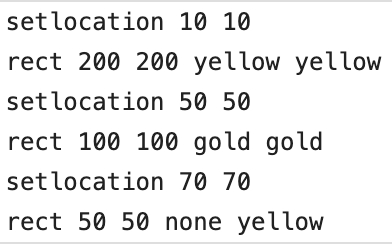
\includegraphics[width=0.3\linewidth]{rect.png}
    \caption{The name of file in examples folder is rect.txt and the output is rect.svg. The above lines of commands saved as a txt file when run with dotnet run rect.txt outputs below:}
    \label{fig:enter-label}
\end{figure}


\begin{figure}[bp!]
    \centering
    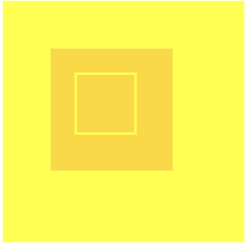
\includegraphics[width=0.3\linewidth]{image.png}
    \caption{Joself Albers similar artwork example}
    \label{fig:enter-label}
\end{figure}

\begin{figure}[bp!]
    \centering
    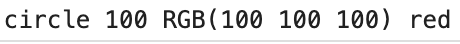
\includegraphics[width=0.3\linewidth]{circleinstructions.png}
    \caption{The name of file in examples folder is circle.txt and the output is circle.svg. The above line of commands saved as a txt file when run with dotnet run circle.txt outputs below:}
    \label{fig:enter-label}
\end{figure}
\begin{figure}[bp!]
    \centering
    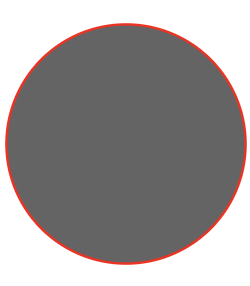
\includegraphics[width=0.3\linewidth]{circle.png}
    \caption{circle}
    \label{fig:enter-label}
\end{figure}


\begin{figure}[bp!]
    \centering
    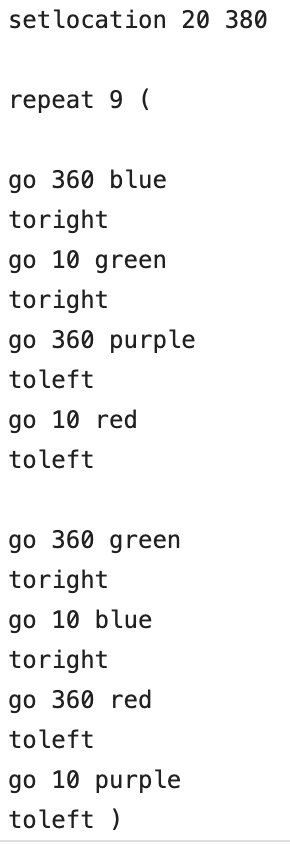
\includegraphics[width=0.3\linewidth]{repeatinglinesinstr.png}
    \caption{The name of file in examples folder is example.txt and the output is example.svg. The above line of commands saved as a txt file when run with dotnet run example.txt outputs below:}
    \label{fig:enter-label}
\end{figure}

\begin{figure}[bp!]
    \centering
    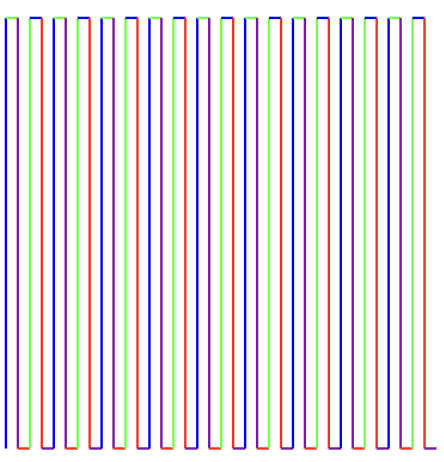
\includegraphics[width=0.3\linewidth]{repeating.png}
    \caption{repeating pattern}
    \label{fig:enter-label}
\end{figure}


\begin{figure}[htbp!]
    \centering
    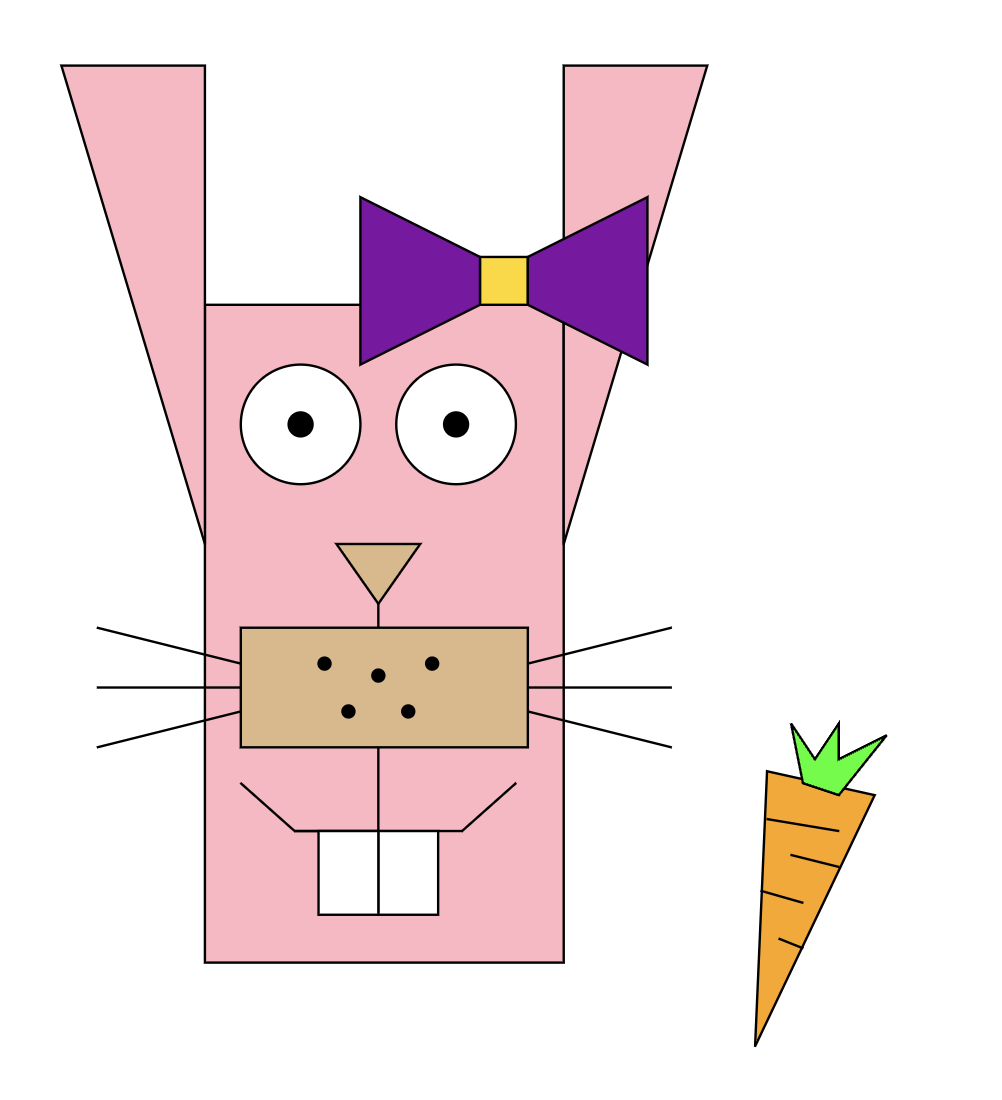
\includegraphics[width=0.5\linewidth]{bunny.png}
    \caption{Image of Bunny using ArtScript}
    \label{fig:enter-label}
\end{figure}

\qquad


% DO NOT DELETE ANYTHING BELOW THIS LINE


\end{document}